\newpage
\chapter{Sensitivity Analysis} \label{ch:sensitivity}

The trade-off tool created to evaluate the concepts is quite complex and has many inter-dependencies. Each of these relations was plotted across a reasonable range of variance against all the significant outputs. Some of the most significant and interesting plots are discussed in this chapter. The trade-off criteria showed little sensitivity for many of the inputs and assumptions plotted. Those plots were either entirely independent of the input, or each of the concepts showed proportional effects, and will have little effect on the trade-off.

\section{Pad Costs}
It was determined that the pad cost could be a major driver of ticket price. The initial assumption was that the ground area needed for the vertiports in downtown LA would have similar cost to office space. If this is the case, over 80\% of the ticket price goes just to these rental fees. This can be seen in \autoref{fig:sens01}. The black x's in the plot show the operating cost without any pad costs. Ideally, better cost arrangements or business models can be developed to subsidise or eliminate the pad cost.

\section{Minimum Trip Range}
By limiting the trip range to a certain minimum, there are two effects that cause the ticket price to drop as shown in \autoref{fig:sens02}. First, the trip efficiency increases if no short trips are allowed (shown in \autoref{fig:sens03}), which reduces energy cost. In addition, due to the calculation method of the tool, a limited trip range means a larger market share is required. Naturally, a larger market share allows for a lower ticket price in the long run. 

\autoref{fig:sens1} shows that, when the minimum range is increased, the total system area increases due to the increased market share. This would increase the pad costs (driving ticket price), but the increased market share still allows for a reduction of the final ticket price. 

When increasing the last-mile penalty, the market share increases, as shown in \autoref{fig:sens2}. Intuitively, it should reduce the market share, as a bigger last-mile penalty would normally decrease demand for flying (as it would take longer to get to and from the vertiport). However, the tool adjusts the market share to meet a standard time savings.

Going forward, the demand must be considered to determine how much market share will be possible in reality. This is an important risk to consider, as it drives the final success of the system. The current tool assumes that demand is essentially infinite, but in reality is likely to be tied directly to trip range and last-mile penalty.


\section{Cruise Altitude}
As expected, the energy required and overall cost increases if a higher cruise altitude is required. This altitude may come from noise and ATC requirements. It is interesting to note that the 2 and 20 passenger vehicles outperform one another depending on this altitude, as shown in in \autoref{fig:sens3}.


\begin{figure}[h]
\begin{subfigure}[t]{0.33\textwidth}
    \centering
    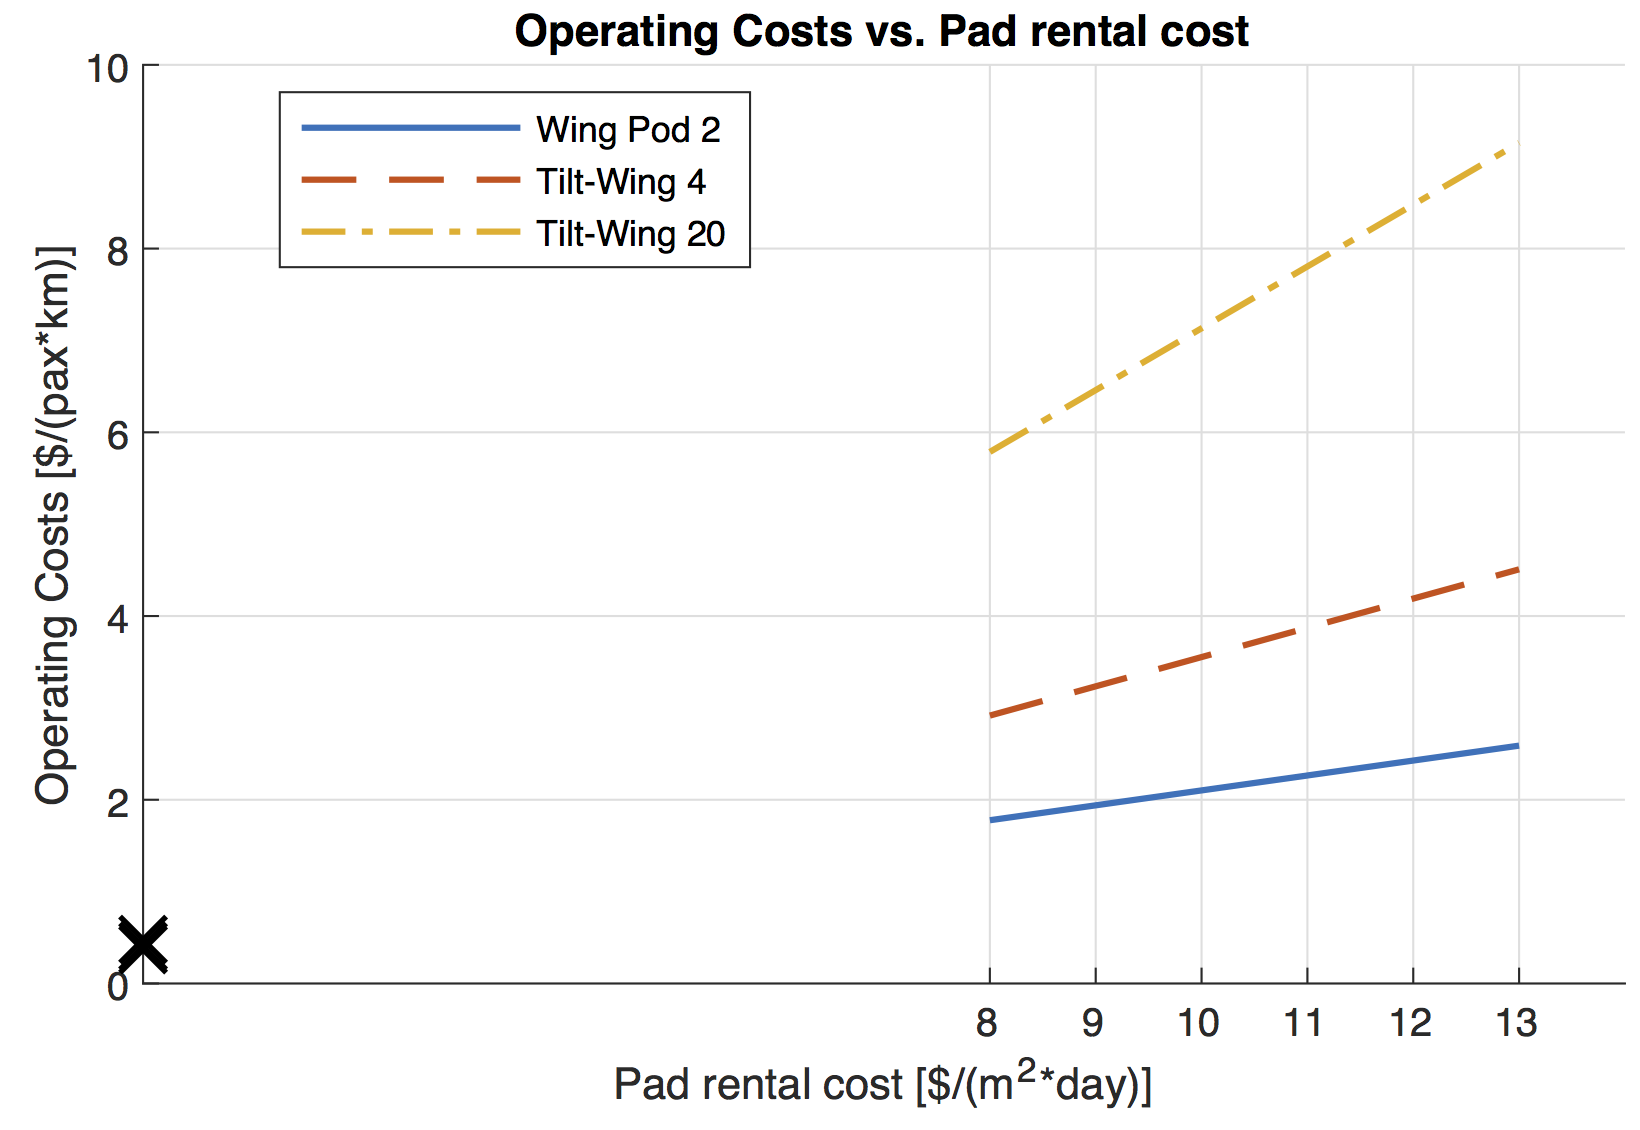
\includegraphics[width=\textwidth]{Figures/cost_oper.png}
    \captionsetup{justification=centering}
    \caption{Total operating cost vs. Pad rental costs}
    \label{fig:sens01}
\end{subfigure}
\begin{subfigure}[t]{0.33\textwidth}
    \centering
    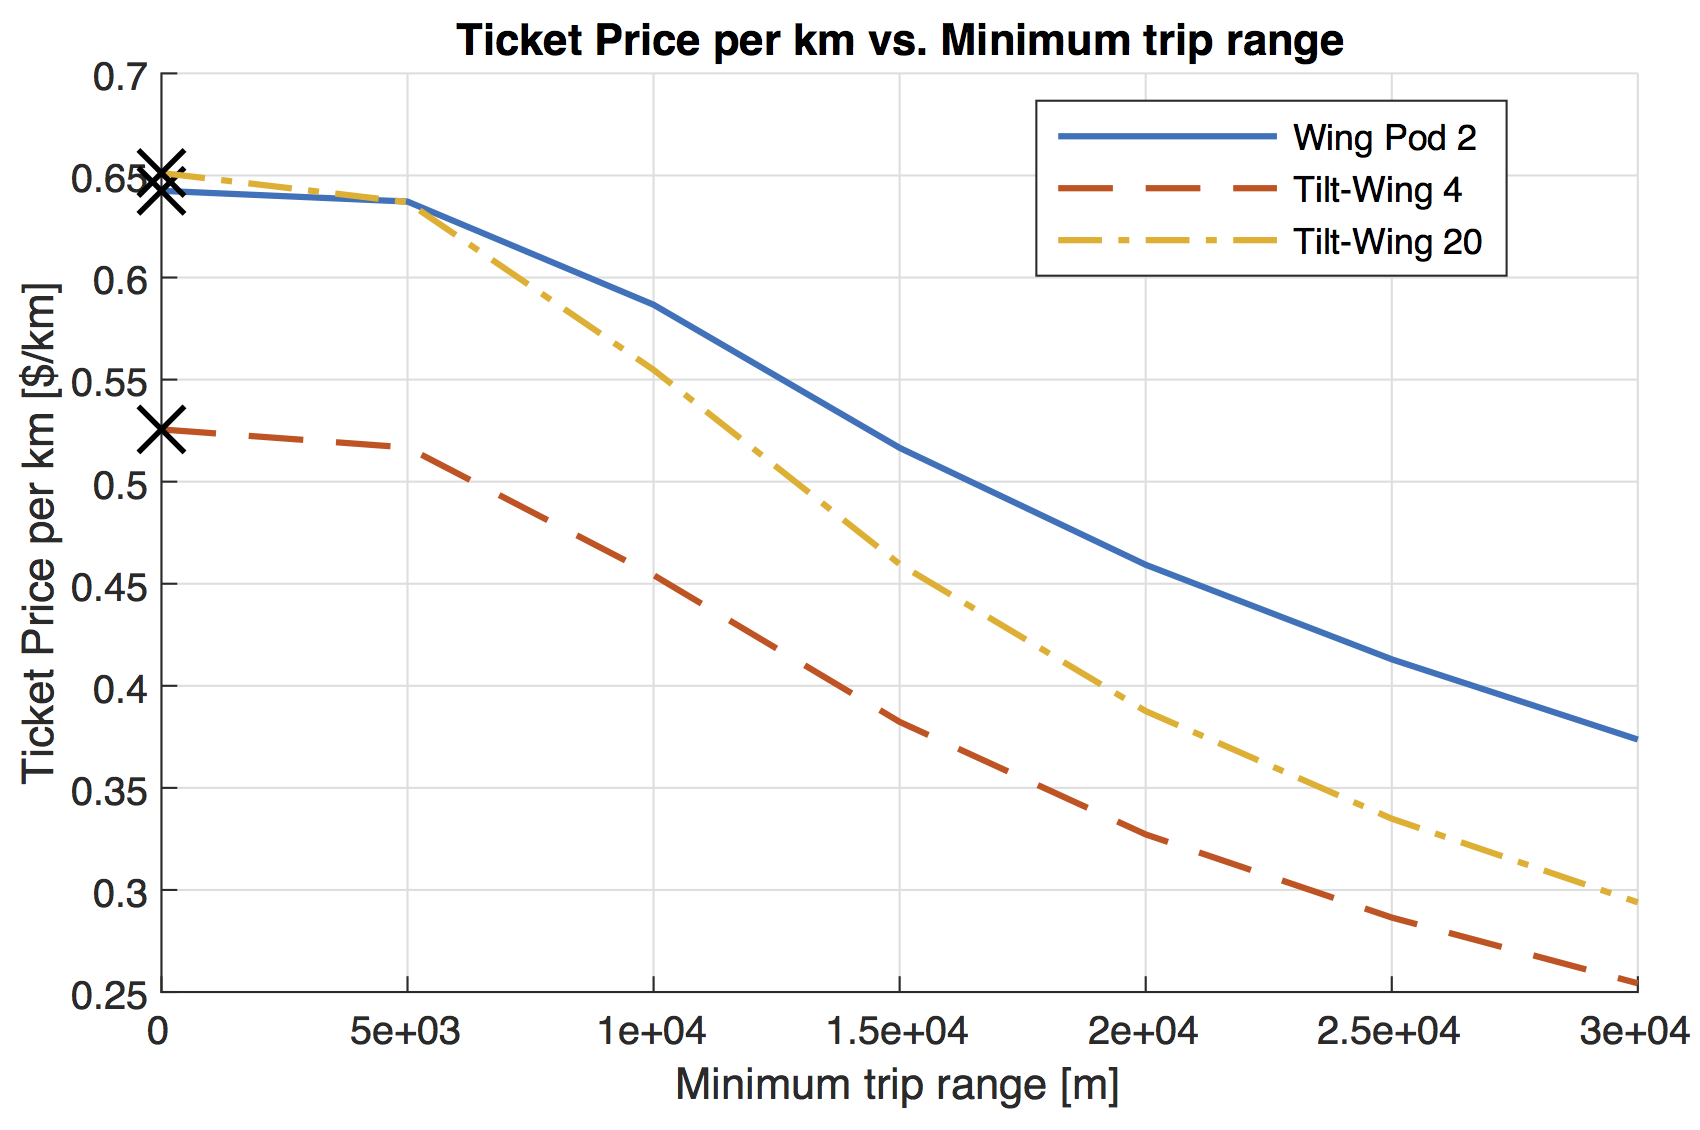
\includegraphics[width=\textwidth]{Figures/minRange_TPrice_perkmNOPAD.png}
    \captionsetup{justification=centering}
    \caption{Ticket price per km vs. Minimum range}
    \label{fig:sens02}
\end{subfigure}
\begin{subfigure}[t]{0.33\textwidth}
    \centering
    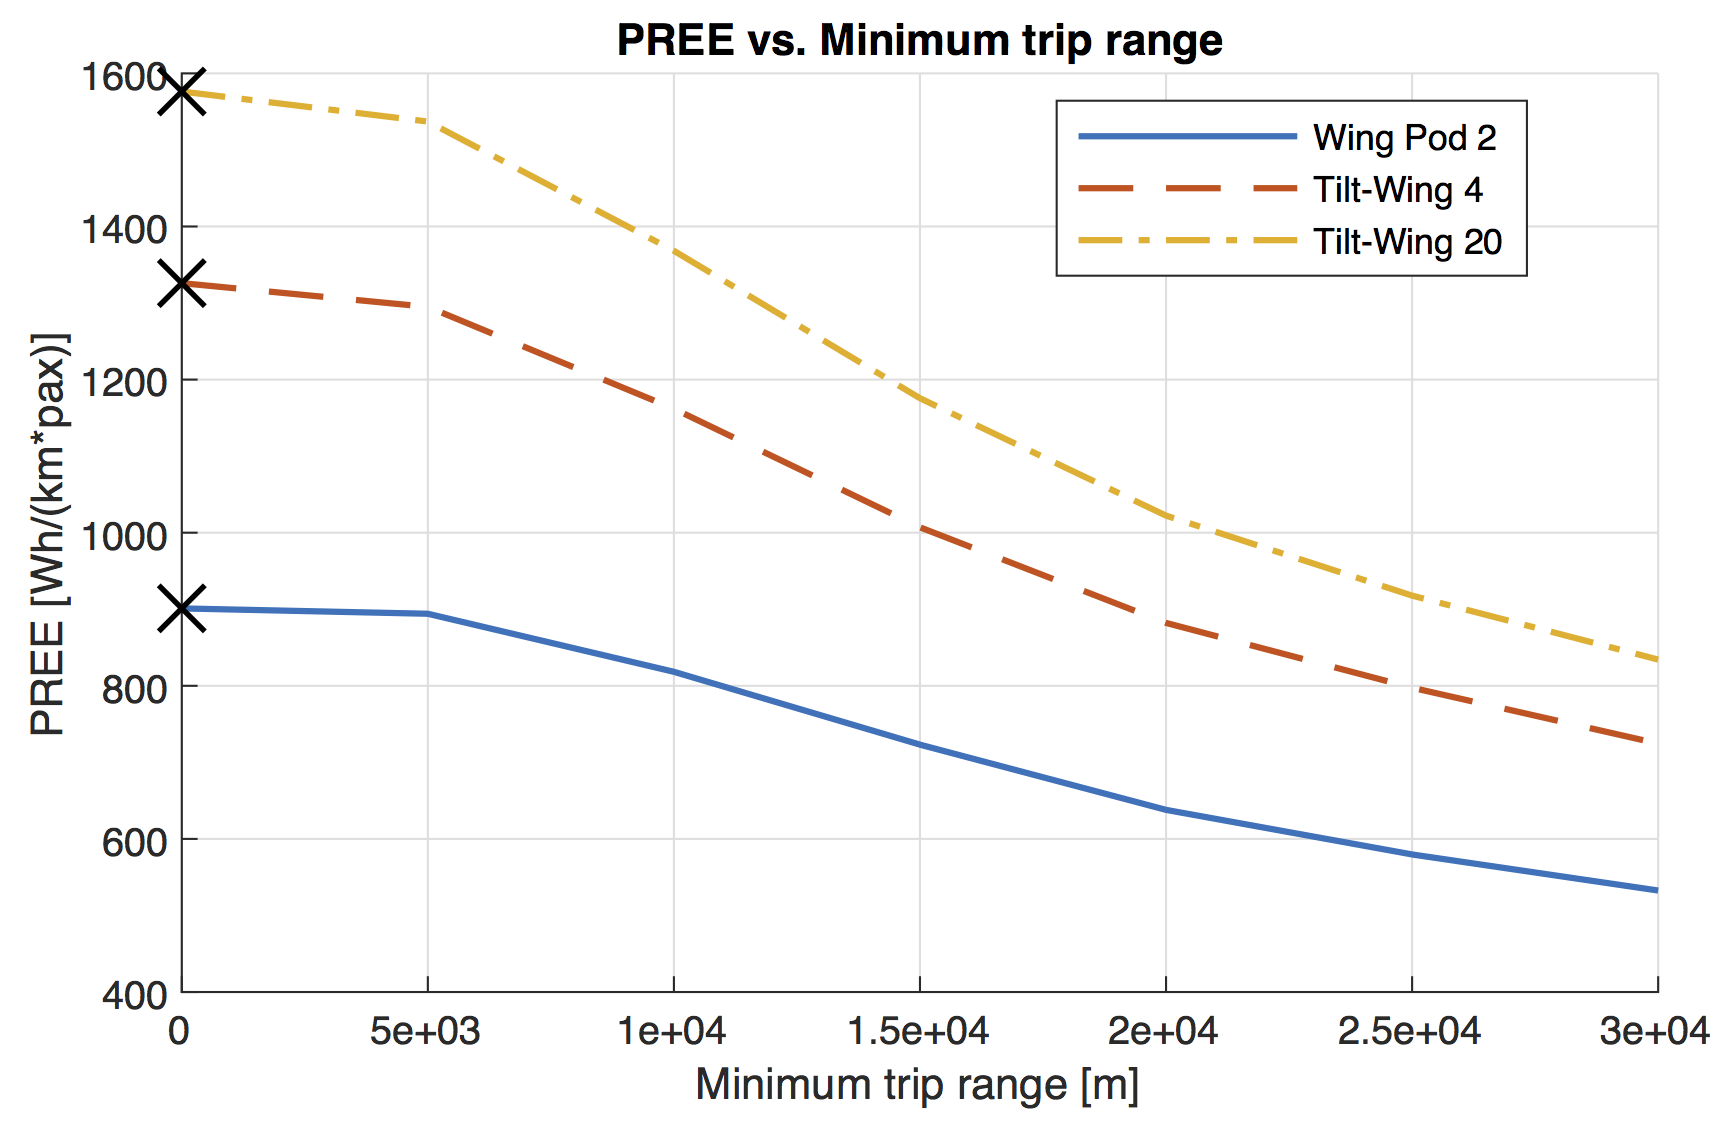
\includegraphics[width=\textwidth]{Figures/report_PREE.png}
    \captionsetup{justification=centering}
    \caption{Passenger range energy efficiency vs. Minimum range}
    \label{fig:sens03}
\end{subfigure}
\captionsetup{justification=centering}
\caption{}
\label{fig:sens0123}
\end{figure}


\begin{figure}[h]
\begin{subfigure}[t]{0.33\textwidth}
    \centering
    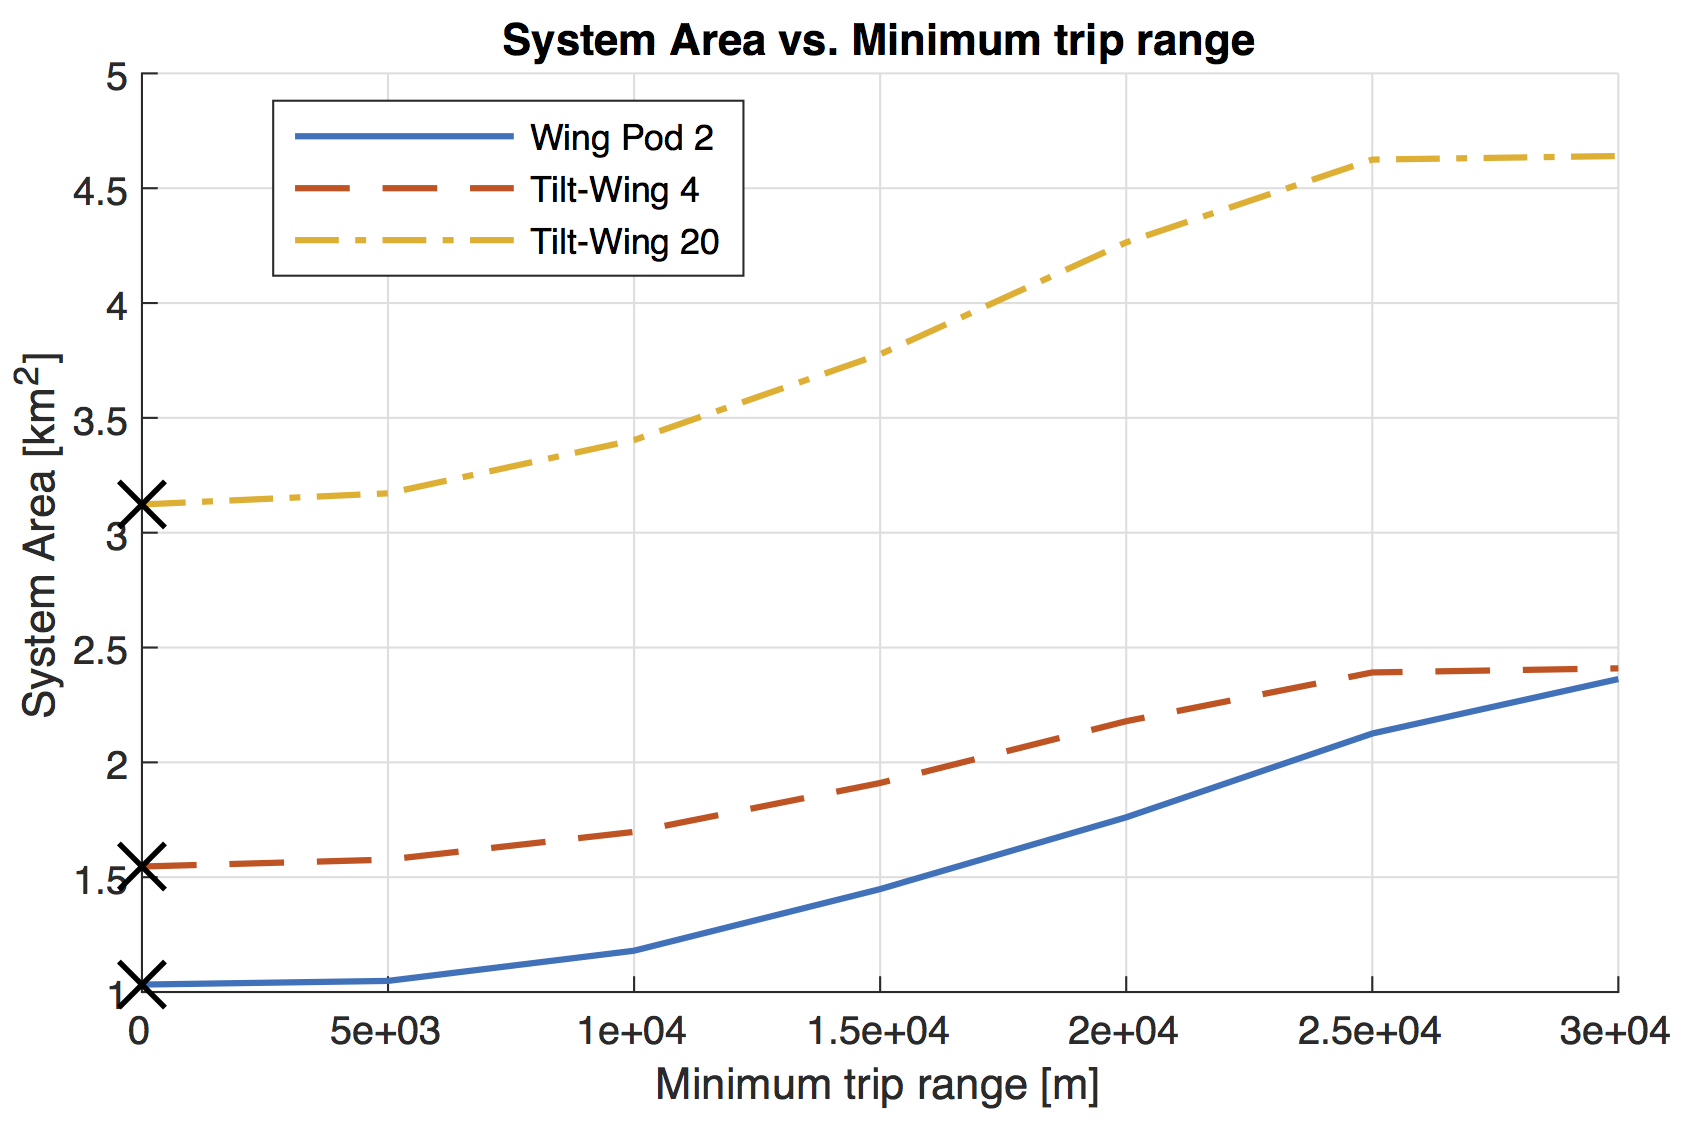
\includegraphics[width=\textwidth]{Figures/report_sys_area.png}
    \captionsetup{justification=centering}
    \caption{Total System Area vs. Minimum Range}
    \label{fig:sens1}
\end{subfigure}
\begin{subfigure}[t]{0.33\textwidth}
    \centering
    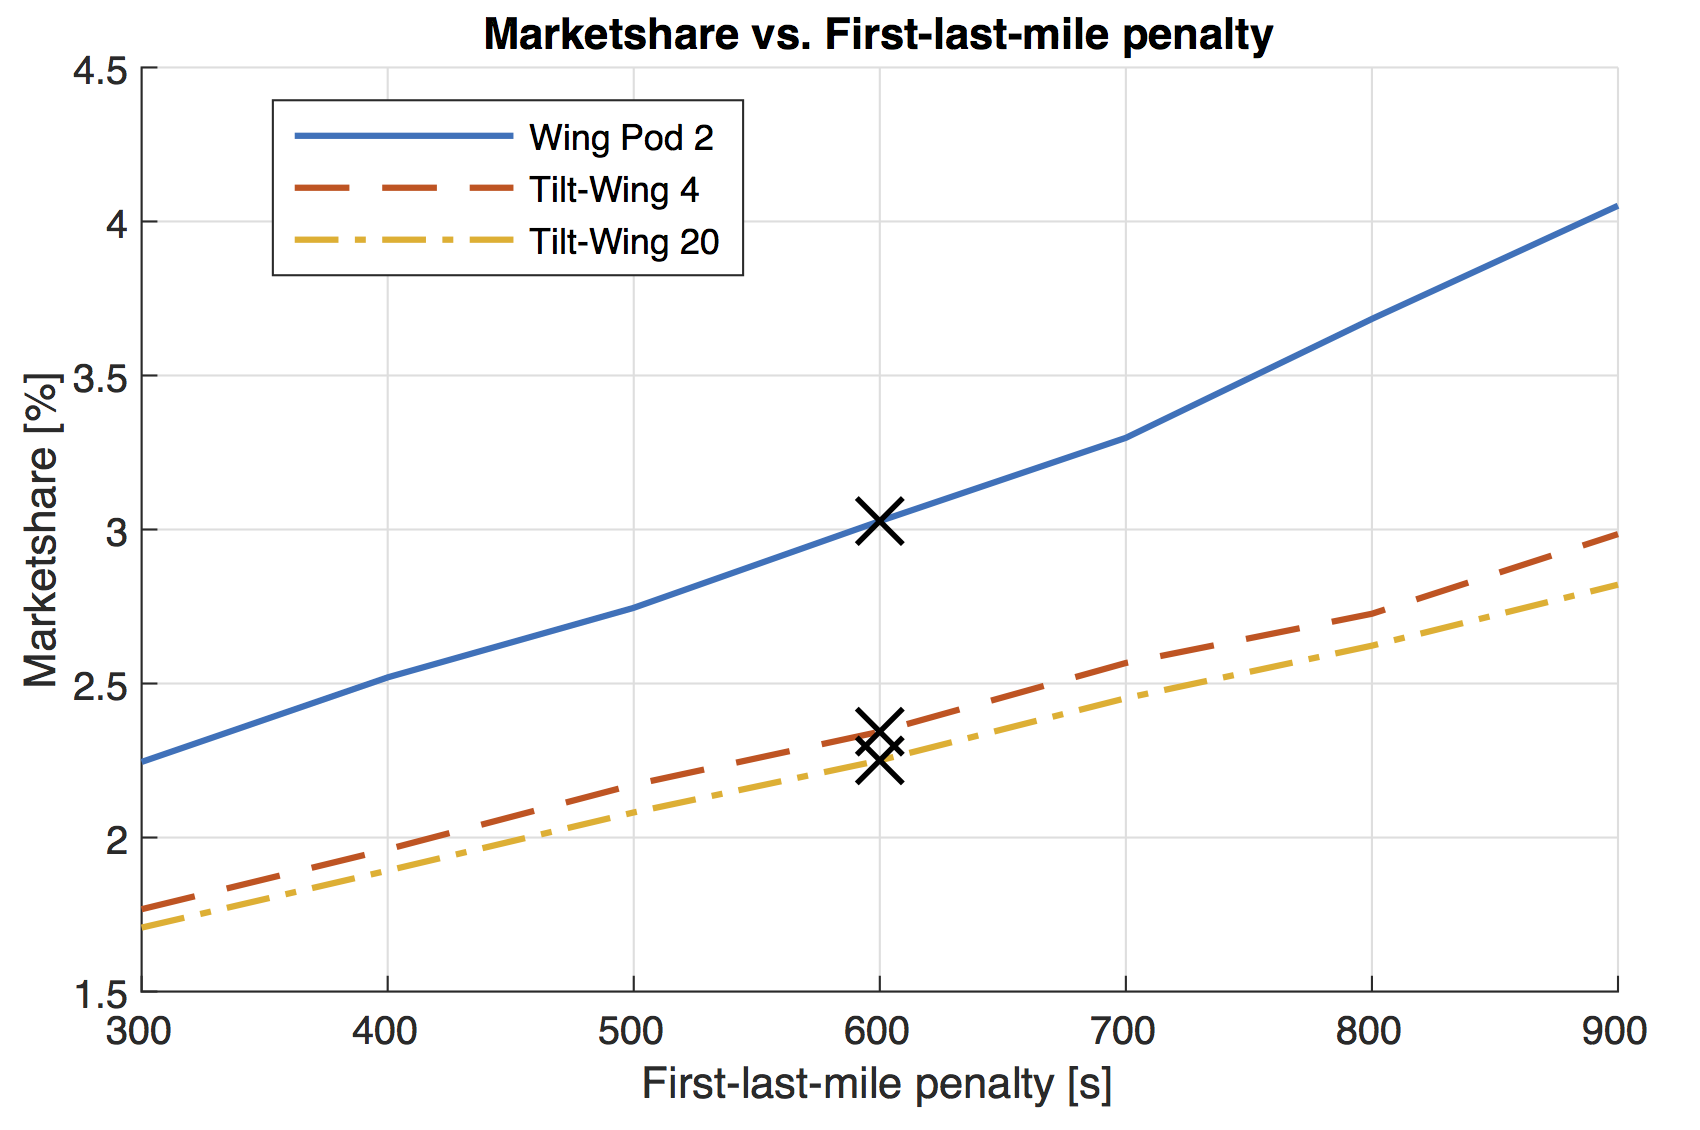
\includegraphics[width=\textwidth]{Figures/report_marketshare.png}
    \captionsetup{justification=centering}
    \caption{Market Share vs. Last-mile penalty}
    \label{fig:sens2}
\end{subfigure}
\begin{subfigure}[t]{0.33\textwidth}
    \centering
    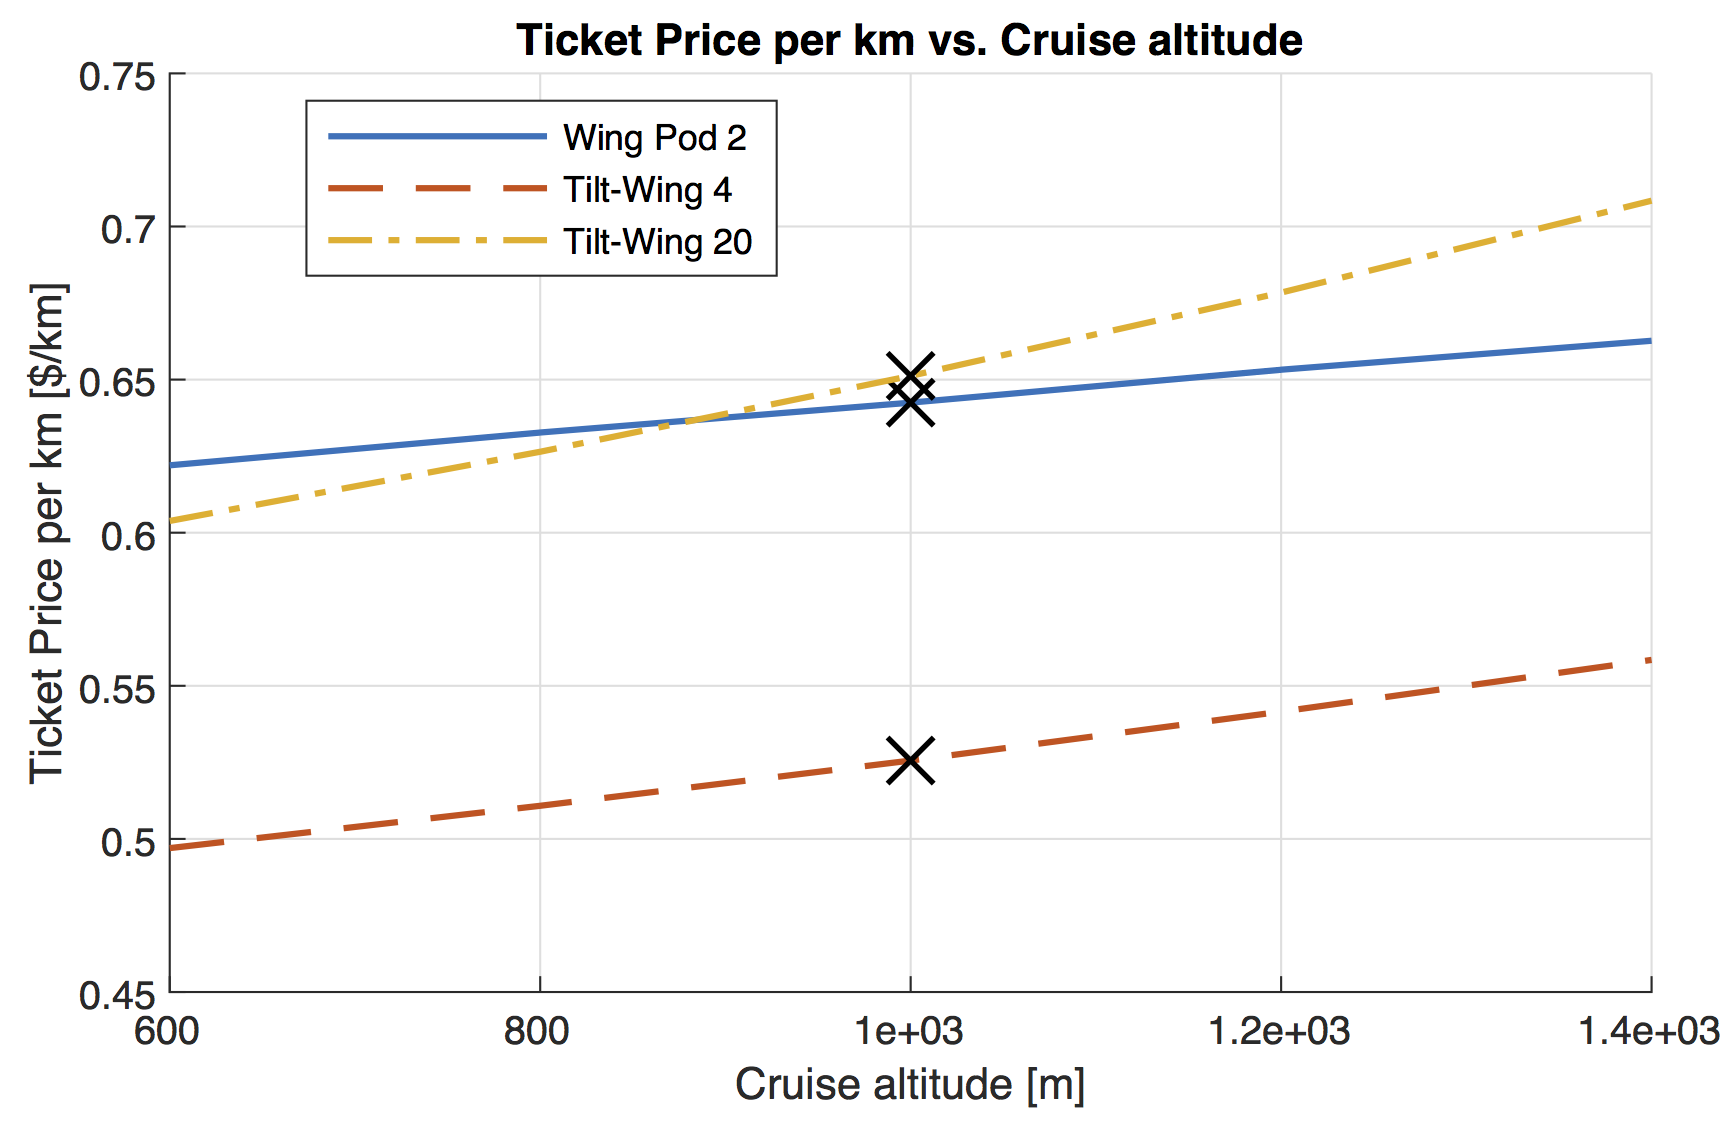
\includegraphics[width=\textwidth]{Figures/Alt_TPrice_perkmNOPAD.png}
    \captionsetup{justification=centering}
    \caption{Ticket price per km vs. Cruise Altitude}
    \label{fig:sens3}
\end{subfigure}
\captionsetup{justification=centering}
\caption{}
\label{fig:sens123}
\end{figure}


\begin{figure}[h]
\begin{subfigure}[t]{0.33\textwidth}
    \centering
    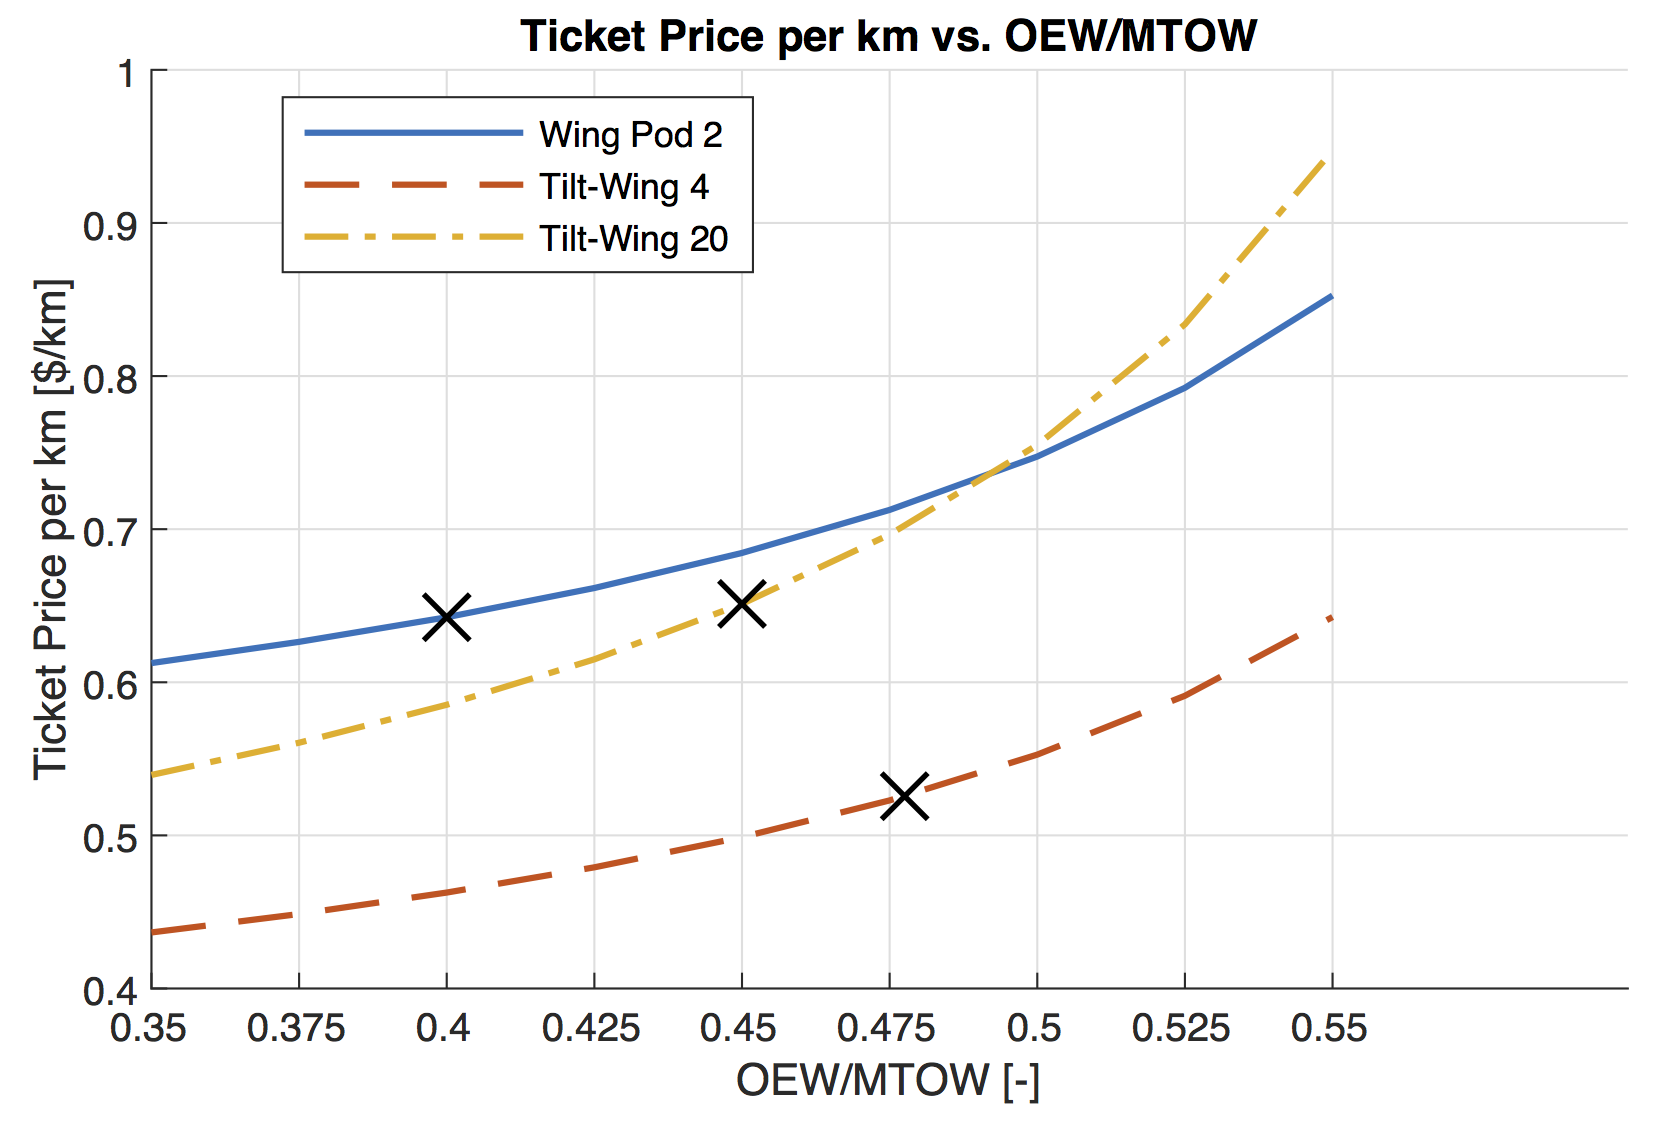
\includegraphics[width=\textwidth]{Figures/OEWMTOW_TPrice_perkmNOPAD.png}
    \captionsetup{justification=centering}
    \caption{Ticket price per km vs. OEW/MTOW ratio}
    \label{fig:sens4}
\end{subfigure}
\begin{subfigure}[t]{0.33\textwidth}
    \centering
    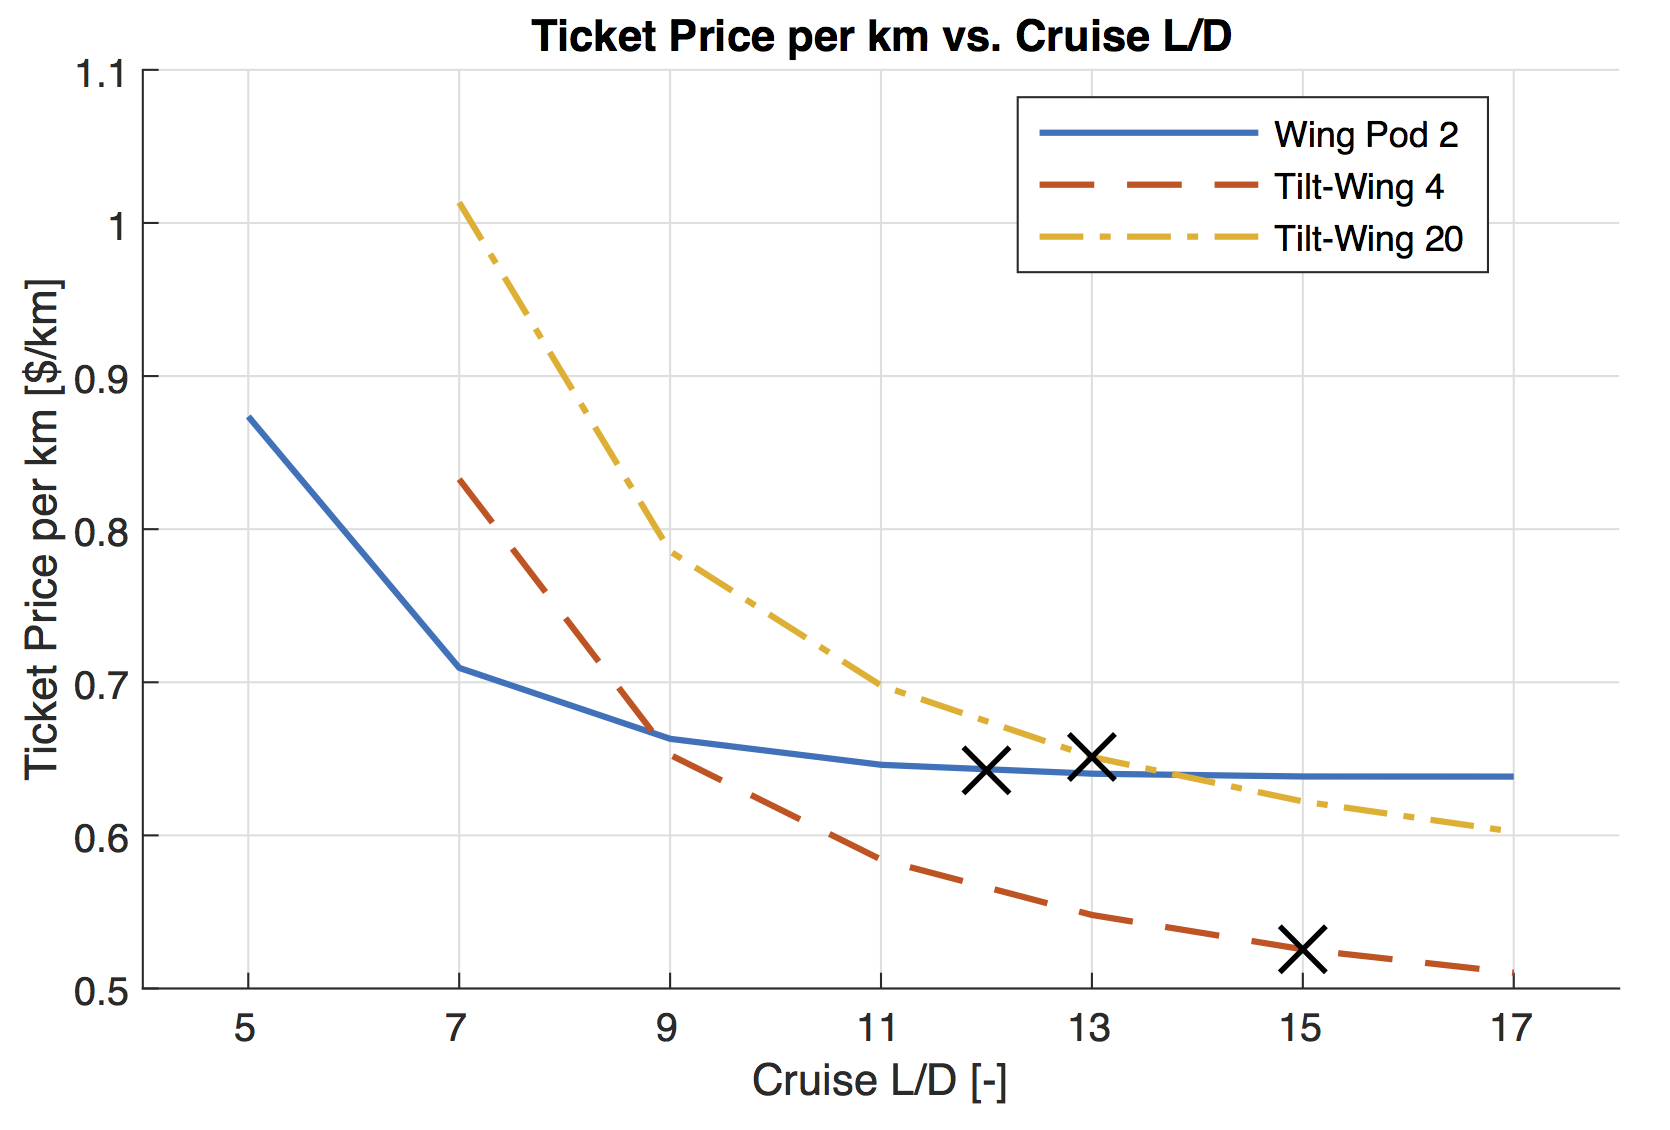
\includegraphics[width=\textwidth]{Figures/LoD_TPrice_perkmNOPAD.png}
    \captionsetup{justification=centering}
    \caption{Ticket price per km vs. L/D in cruise}
    \label{fig:sens5}
\end{subfigure}
\begin{subfigure}[t]{0.33\textwidth}
    \centering
    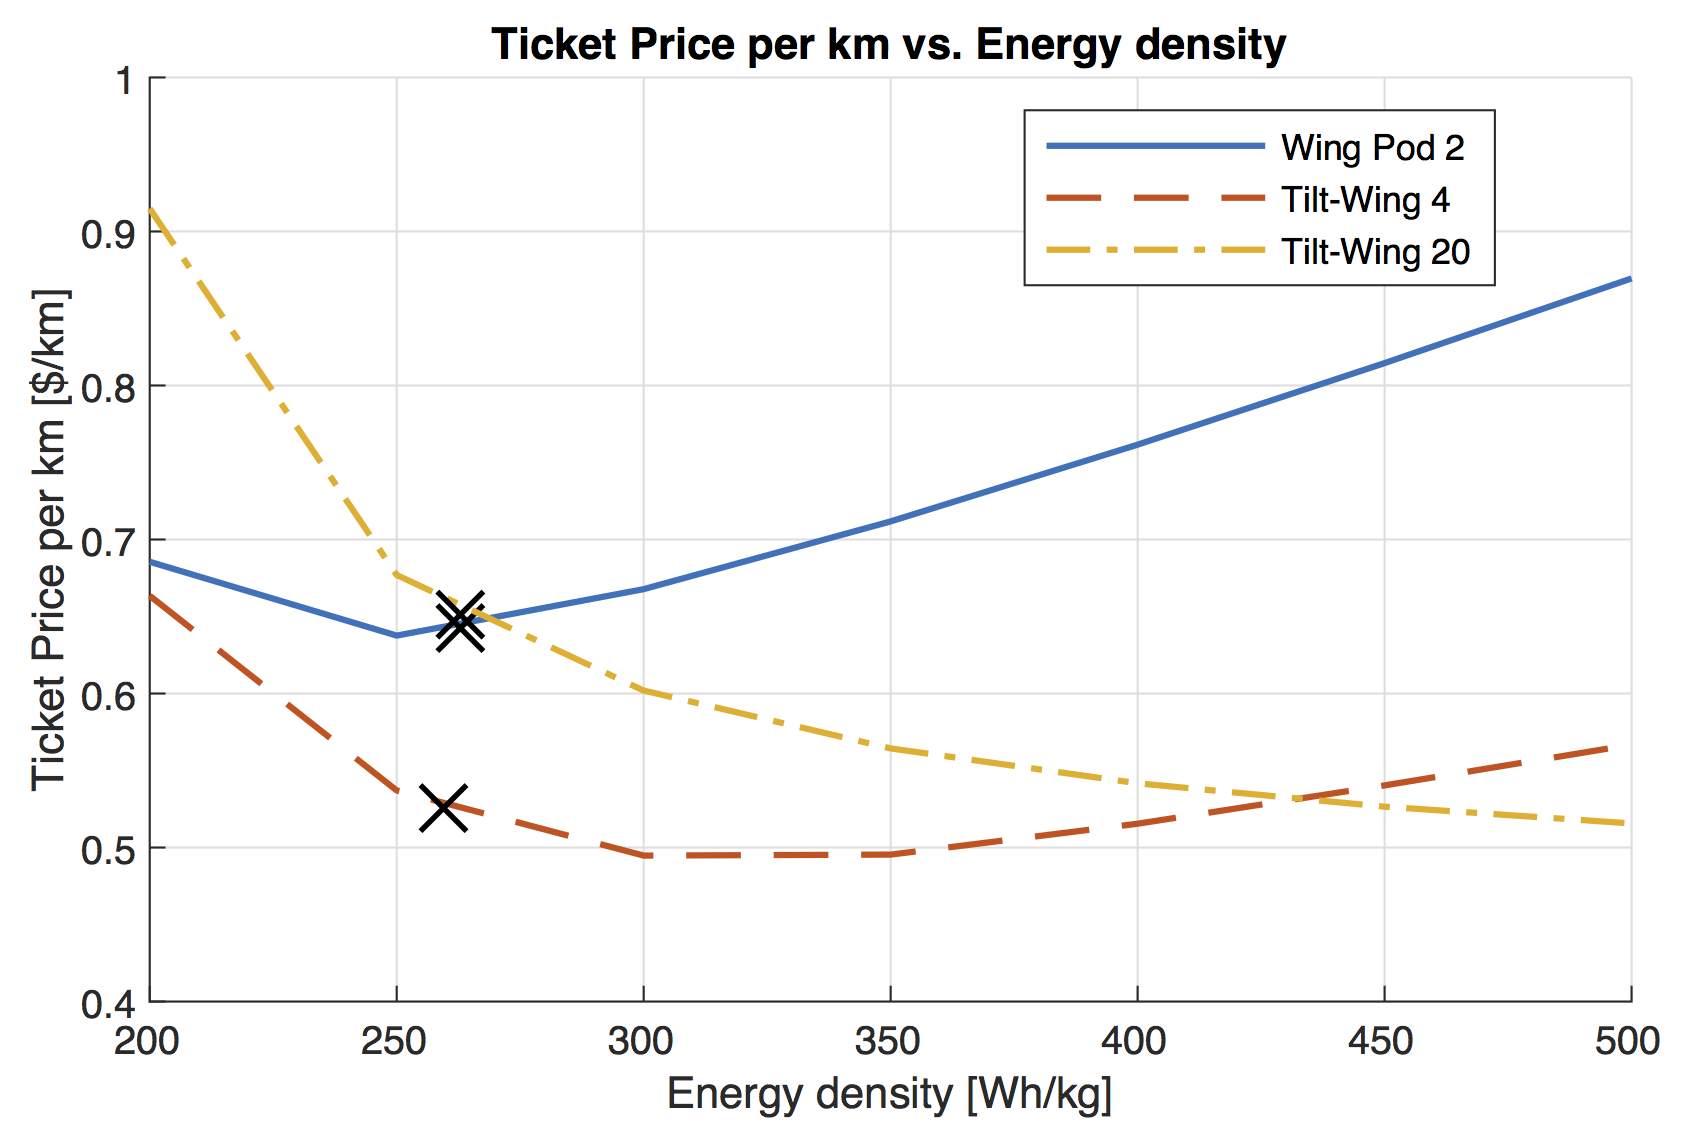
\includegraphics[width=\textwidth]{Figures/Edens_TPrice_perkmNOPAD.png}
    \captionsetup{justification=centering}
    \caption{Ticket price per km vs. Battery energy density}
    \label{fig:sens6}
\end{subfigure}
\captionsetup{justification=centering}
\caption{}
\label{fig:sens456}
\end{figure}

\begin{figure}[h]
\begin{subfigure}[t]{0.33\textwidth}
    \centering
    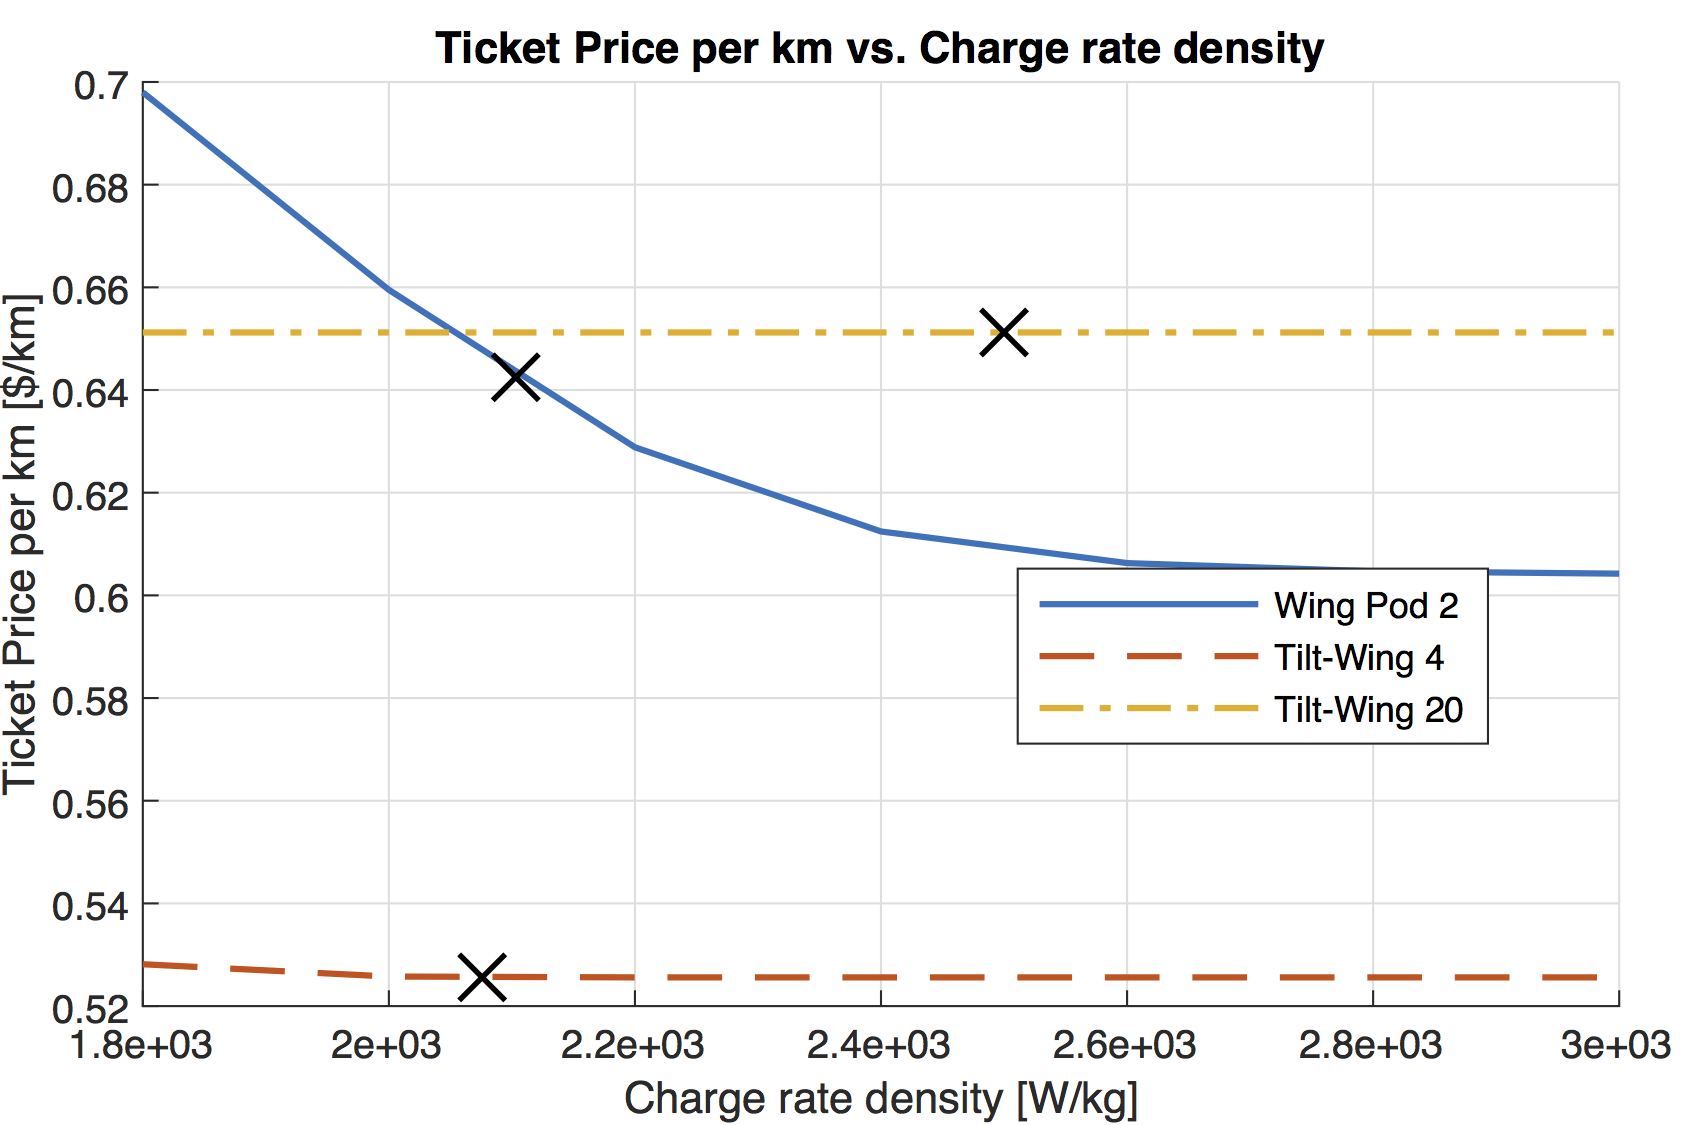
\includegraphics[width=\textwidth]{Figures/CRate_TPrice_perkmNOPAD.png}
    \captionsetup{justification=centering}
    \caption{Ticket price per km vs. Charge rate density}
    \label{fig:sens7}
\end{subfigure}
\begin{subfigure}[t]{0.33\textwidth}
    \centering
    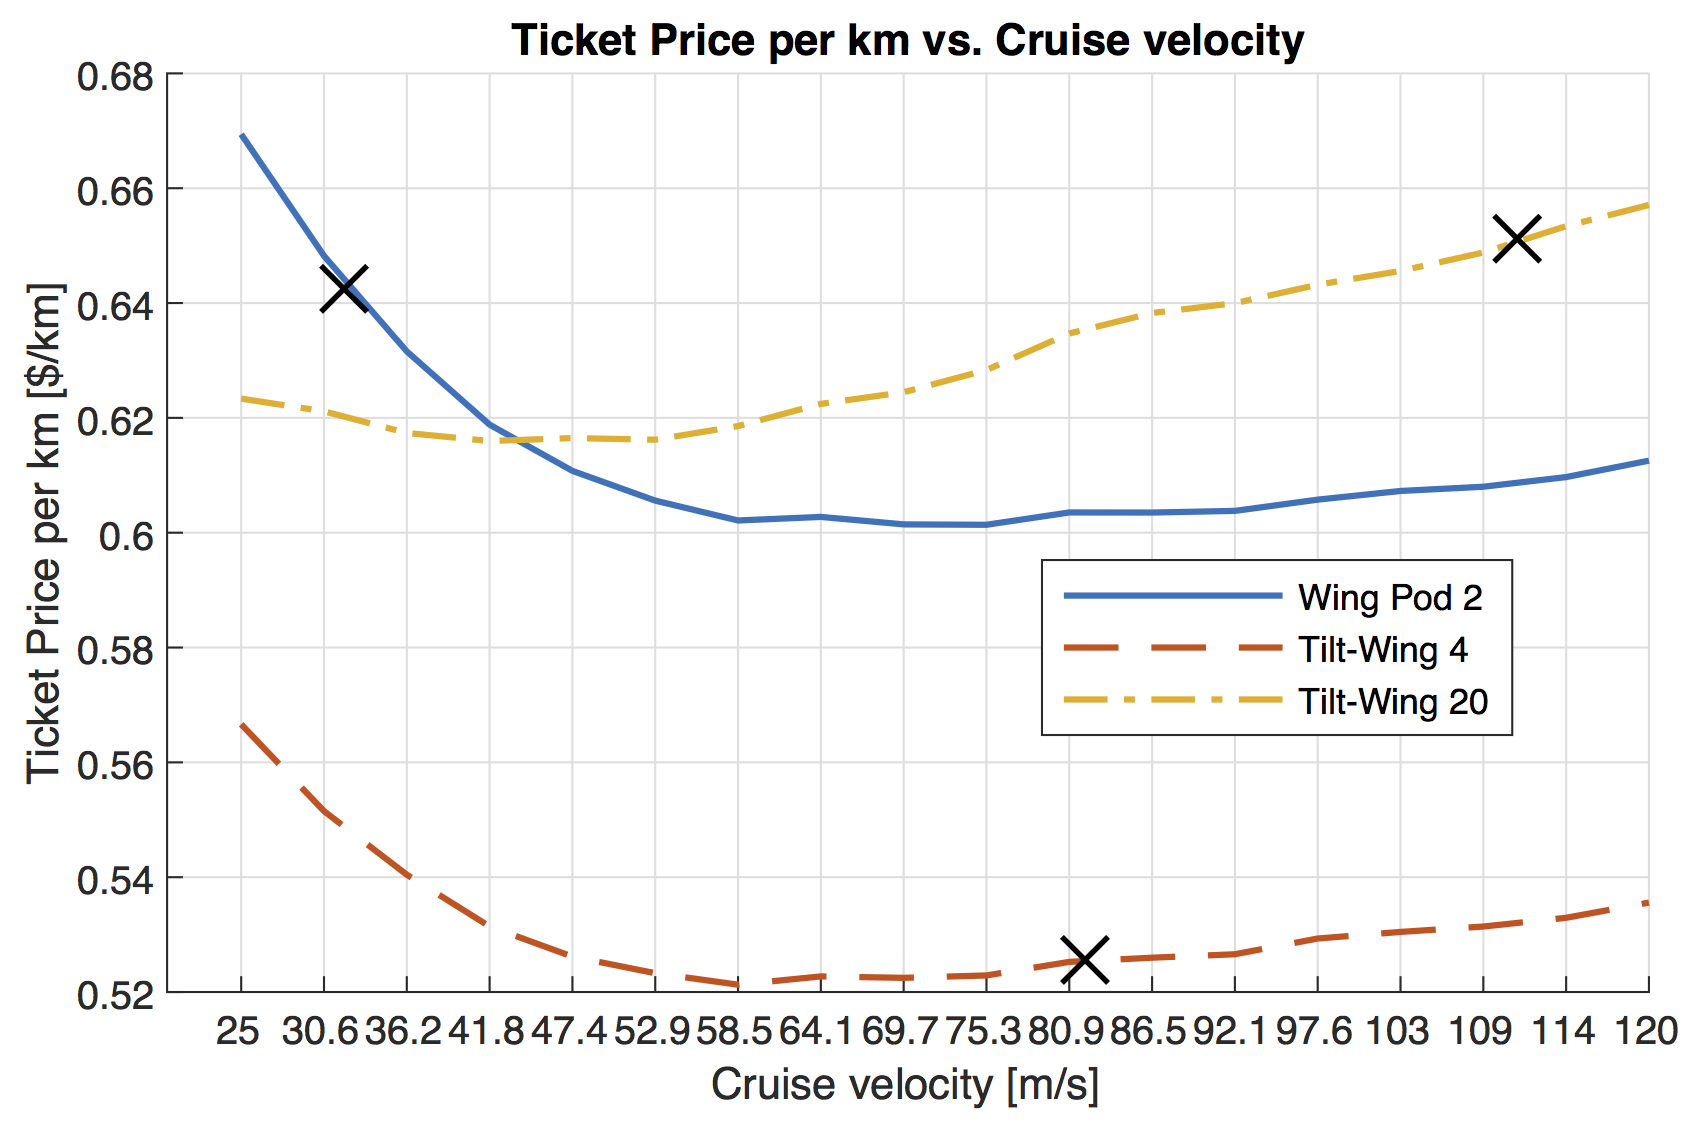
\includegraphics[width=\textwidth]{Figures/Cruise_TPrice_perkmNOPAD.png}
    \captionsetup{justification=centering}
    \caption{Ticket price per km vs. Cruise velocity}
    \label{fig:sens8}
\end{subfigure}
\begin{subfigure}[t]{0.33\textwidth}
    \centering
    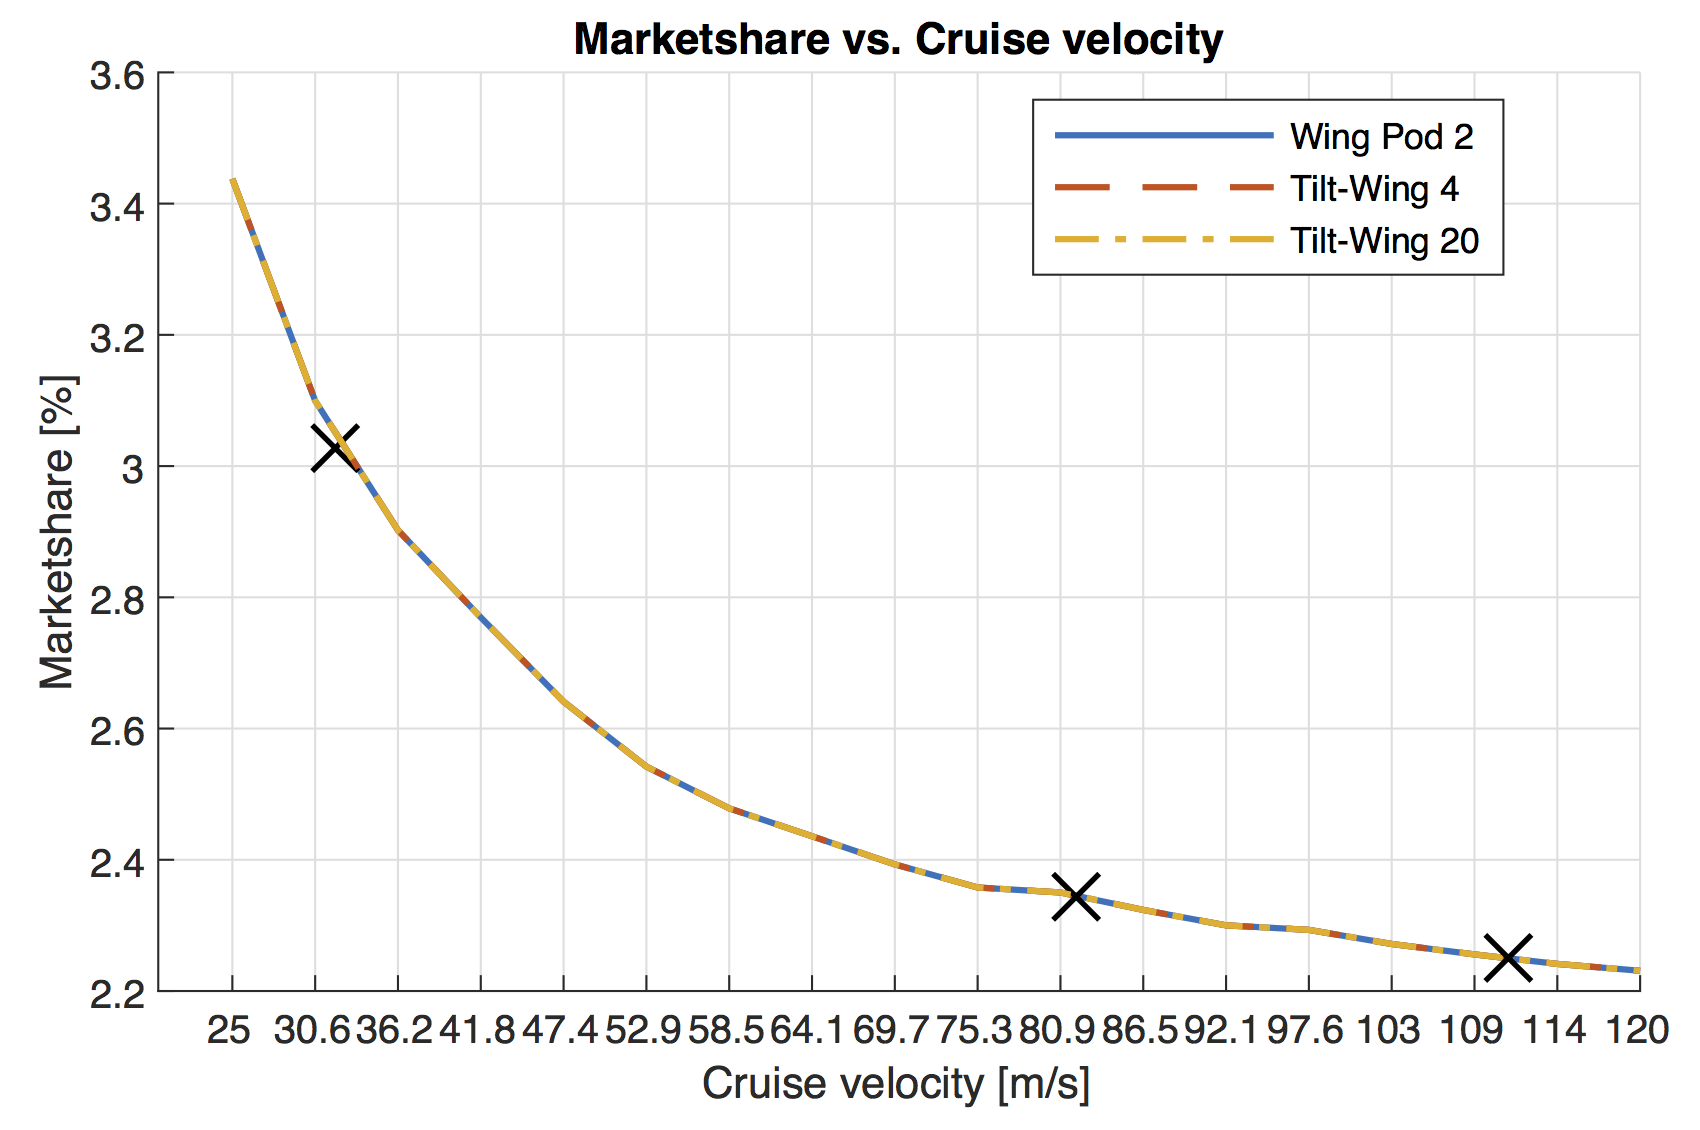
\includegraphics[width=\textwidth]{Chapters/cruise_marketshare.png}
    \captionsetup{justification=centering}
    \caption{Market share vs. Cruise velocity}
    \label{fig:sens9}
\end{subfigure}
\captionsetup{justification=centering}
\end{figure}

\section{Vehicle Weight and Energy Consumption}
Some sensitivities are intuitively explained and verify the correct working of the tool. For example, an increase in the fraction of empty and maximum operational mass causes a higher ticket price. The heaviest vehicle is effected most by that effect as can be told by comparing the slopes in figure \ref{fig:sens4}. A more efficient cruise causes the energy consumption to be lower which also decreases OEW (OEW is considered an output of the tool here, since it is converged on every run). 

Counterintuitive is that ticket price can increase with increasing energy density. This does not seem to make sense at first. However, consider that charge rate density (expressed in W/kg) is kept constant when energy density is perturbed. Recall, that the batteries recharging time is modelled as inversely proportional to the charge rate and proportional to the energy needed for every given trip. Since the chosen vehicles are energy limited (not power limited) during take off, this means that battery mass decreases as energy density increases. However, the trip energy demand does not vary linearly with the battery mass. It varies approximately as $MTOW\sqrt{MTOW}$ during the hovering phases, as opposed to the charge rate, which \emph{is} inversely proportional to the battery mass \autoref{eq:power}. This way, charge time actually increases, because the increase in charge rate with battery mass is lower than the increase in energy demand with battery mass. Therefore, a longer turnaround time is needed for recharging which necessitates a bigger fleet and more vertiports for the same passenger throughput. This means that we will have to find battery technology that does not just increase energy density, since a smaller battery does not necessarily improves economic performance; a very interesting result. The reason that the 20 person vehicle in \autoref{fig:sens6} is not following this trend is because the turnaround time is limited by boarding procedures, not charging time. So a longer charging time does not deteriorate ticket price. The bottom line to this is that optimisation for the smallest necessary battery weight, as done in tool, may not yield the lowest ticket price even if it improves sustainability through less battery mass and lower energy usage per passenger kilometre.

Also; not shown here, the system area increases for a higher L/D. If pad infrastructure costs are higher than shown here, the sensitivity in L/D can reverse. So a higher L/D actually increases ticket prices, if optimisation for the lightest possible MTOW is performed, as usual. Compare with \autoref{fig:sens5}.


\begin{wrapfigure}[18]{r}{0.35\textwidth}
    \centering
    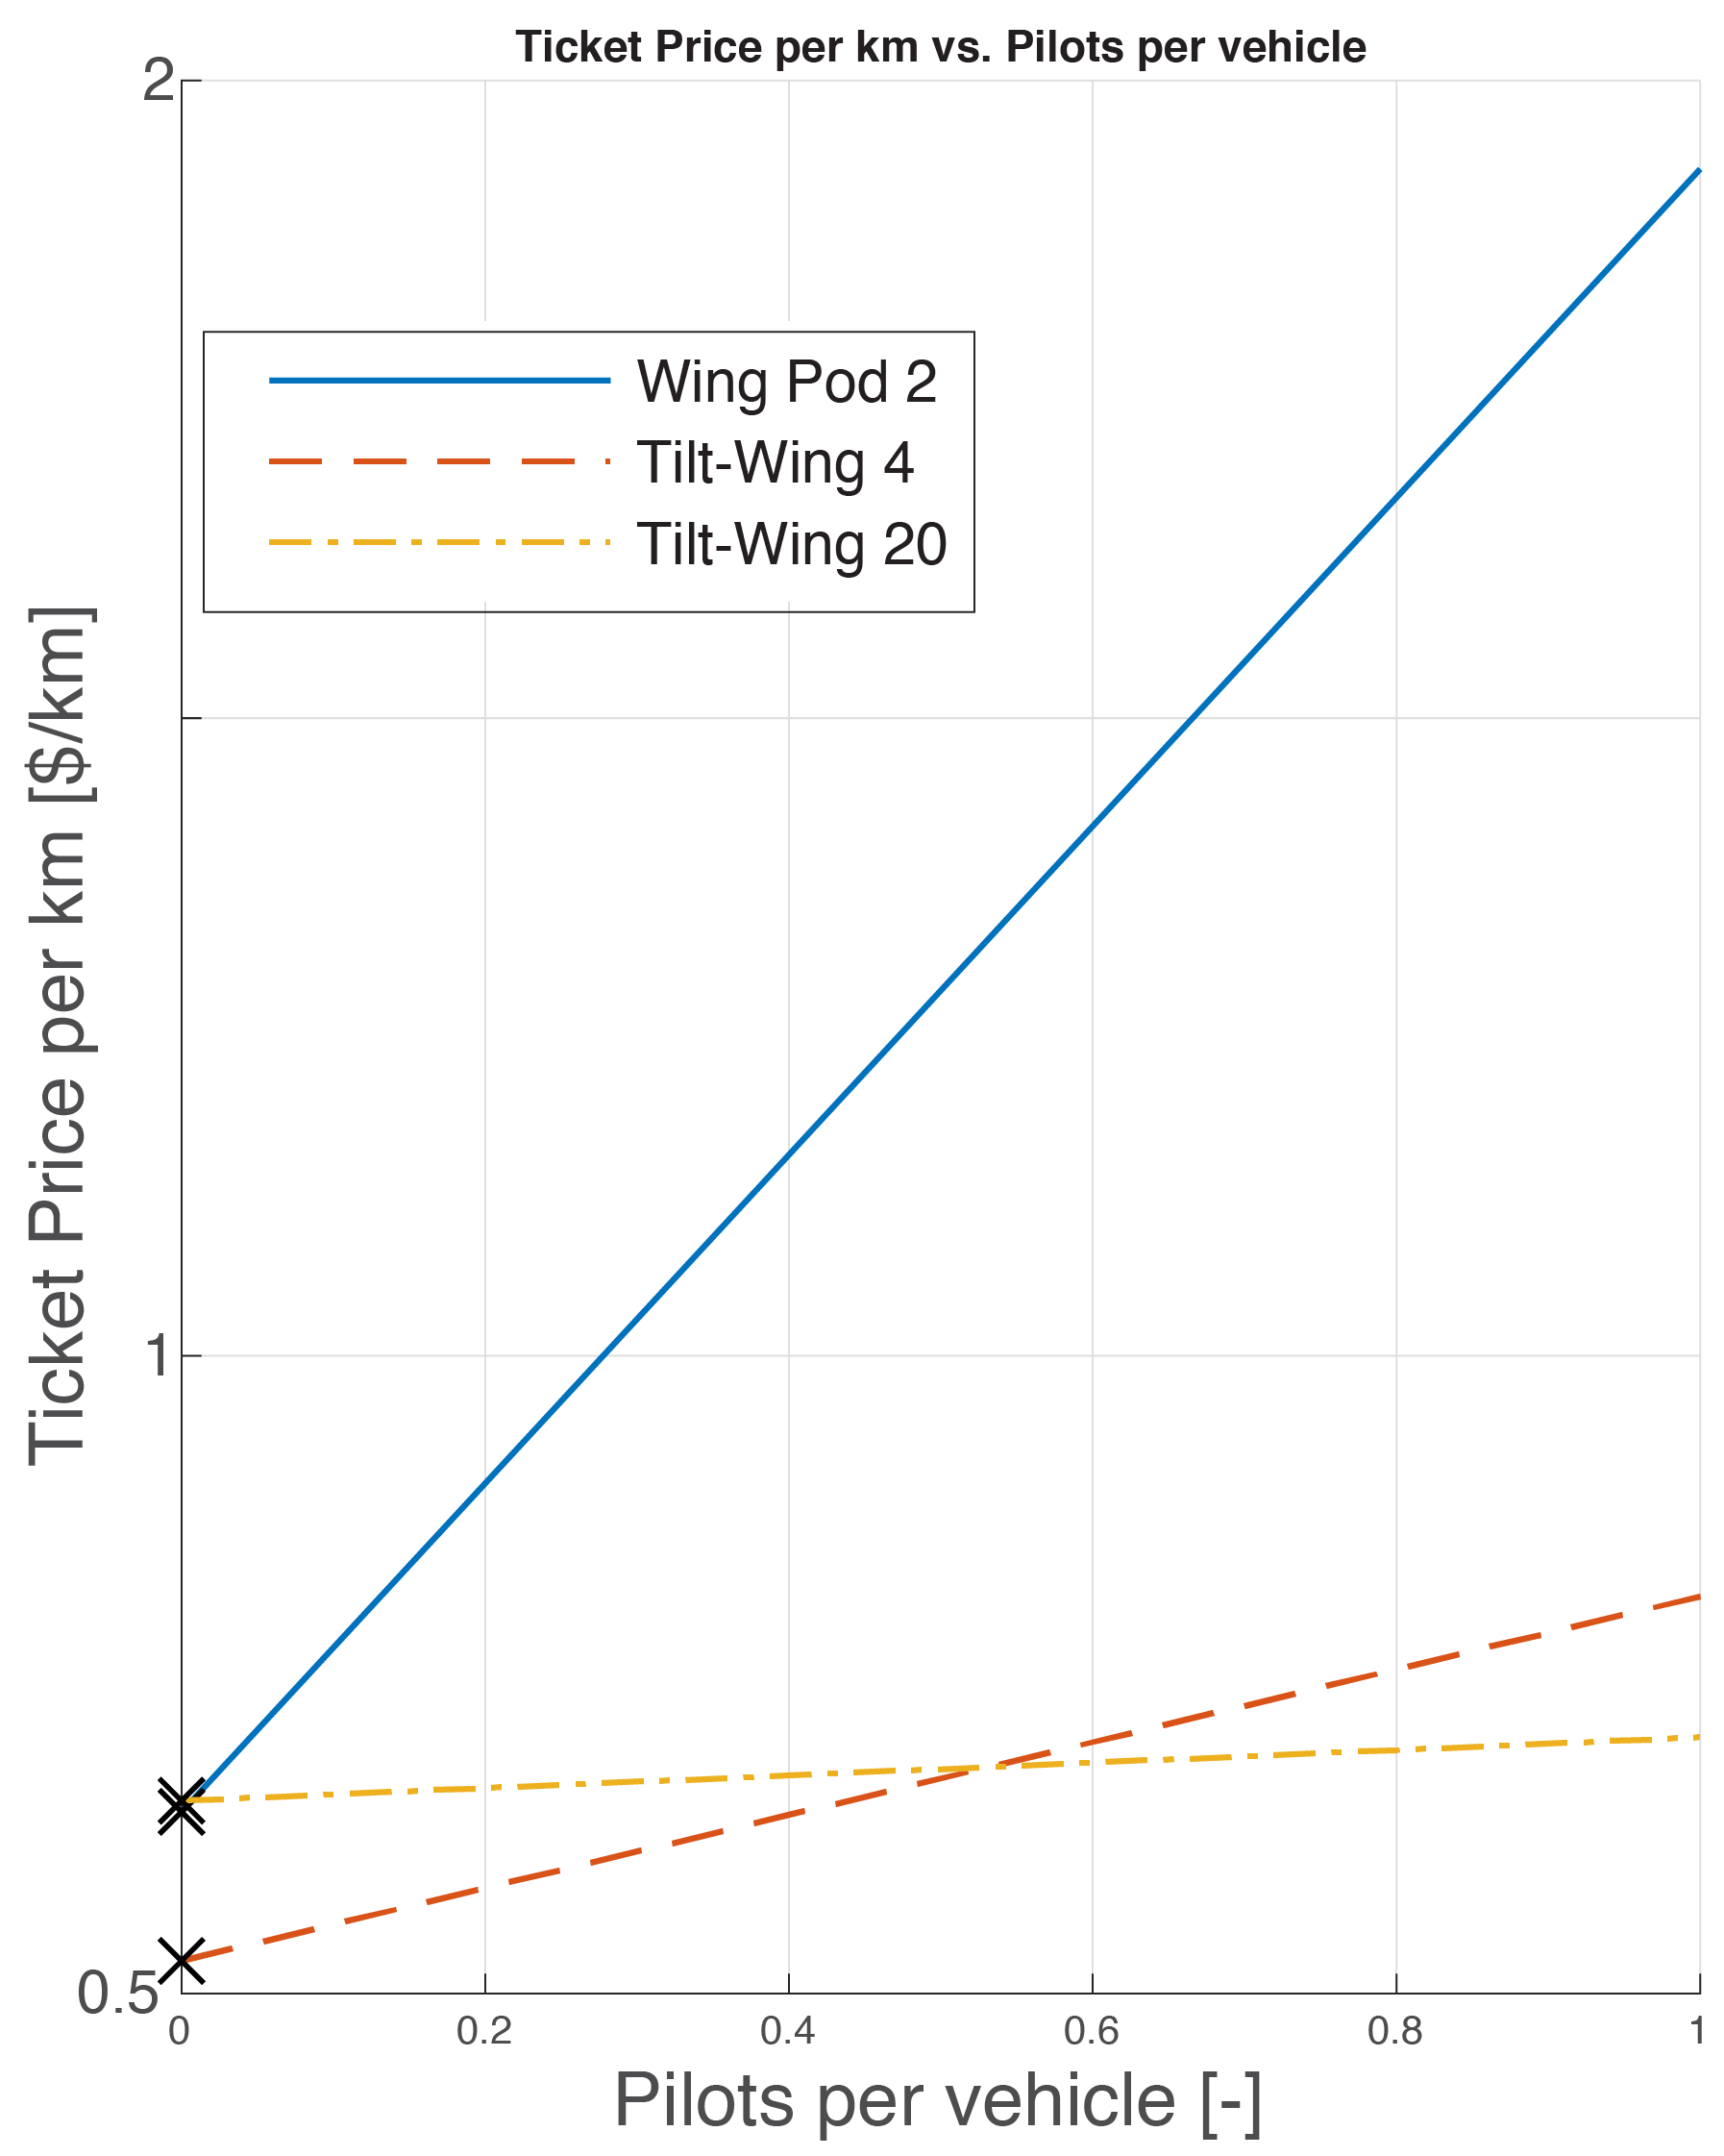
\includegraphics[width=0.35\textwidth]{Figures/autonomous_TPrice_perkm.png}
    \captionsetup{justification=centering}
    \caption{Ticket price increase due to including remote pilots, to assist autonomous vehicles.}
    \label{fig:autocost}
\end{wrapfigure}

\section{Cruise Velocity}
The cruise velocity is dependent on the vehicle design and has an important impact on the ticket price, due to its link with travel time. The ticket price change shown in \autoref{fig:sens8} is partly due to the change in market share (shown in \autoref{fig:sens9}). The shape of the plots are determined by the market share, but their translation is due to other sensitivities. Fortunately, there is a stand-out winner that may override those sensitivities.

\section{Autonomous and Remotely Assisted Piloting}
Much of the trade-off has been done assuming that all the vehicles are completely autonomous. It is likely that remote piloting capabilities will be necessary for safety reasons. A pilot may need to intervene in certain situations. This also helps with a feeling of comfort for passengers. These pilots cost money, and will increase the operating cost per vehicle. By completing a sensitivity study based on the number of remote pilots, it can be shown at what point one concept may cost less than another. \autoref{fig:autocost} shows that the large vehicle benefits the most, and becomes cheaper (per km) to operate than the 4 passenger at 0.5 (1 pilot for every 2 vehicles). It seems more likely that less pilots will be required though.
